\documentclass[a4paper,11pt]{book}
\usepackage[T1]{fontenc}
\usepackage[utf8]{inputenc}
\usepackage{lmodern}
\usepackage{url}
\usepackage{graphicx}
\usepackage[UKenglish]{babel}
\usepackage[UKenglish]{isodate}

\addto{\captionsspanish}{\renewcommand{\chaptername}{Chapter}}
\addto{\captionsspanish}{\renewcommand{\appendixname}{Appendix}}
\addto{\captionsspanish}{\renewcommand{\indexname}{Appendix}}
\addto{\captionsspanish}{\renewcommand{\contentsname}{Appendix}}
\addto{\captionsspanish}{\renewcommand{\bibname}{Bibliography}}

\title{MUSES Developer Guide}
\author{Sweden Connectivity AB, S2 Grupo, University of Granada, \\HiTec, University of Geneva}
\cleanlookdateon

\begin{document}

\maketitle
\tableofcontents

\chapter{Introduction}
\label{ch:intro}

This guide describes everything a developer needs to know to start developing for the MUSES system.

The MUSES System \cite{deliverable21} has been developed based on the client-server architecture. 
 
The client or device is related to the end user, usually an employee who uses a mobile or a portable device possibly
personal device to access enterprise resources. From the enterprise security point of view, the system should prevent the user from using the device incorrectly and make sure that the employee follows the company policees. Therefore, MUSES monitors the user's context and behaviour, and controls their actions, allowing or forbidding them depending on company policies.

The MUSES server is controlled by an enterprise security manager, the Chief Security Officer (CSO), who defines the security policies to be considered in the MUSES system. The security policies are used by the MUSES server to identify which behaviour is allowed and which one is not. The server then receives, stores, and processes all the gathered information from users' devices. After that, it analyzes the data, performing a real-time risk and trust analysis. In addition, the system detects policy violations through event correlation techniques, adapting to changes in the environment, as well as non-secure user behaviours.

\section{MUSES on Github}
\label{sec:musesgit}

All the MUSES system code is available at \url{https://github.com/MusesProject}. That is the Github organisation page for MUSES, and it contains the following repositories:

\begin{description}
  \item[Muses-Developer-Guide] Repository with the TeX files which consist of a manual for users that may want to develop for the MUSES project.
  \item[Muses-Security-Quiz] Contains the first version of the Spring roo project that implements the Security Quiz for MUSES project.
  \item[MusesCommon] This repository contains the java classes which are common for client and server projects, to reduce duplication of classes in projects.
  \item[MusesServer] This repository contains all the files in the Java-Maven MUSES server project.
  \item[MusesClient] Repository containing the first prototype of the MUSES client, developed for Android.
  \item[MusesSituationPredictionStudy] Contains the very first prototype of an Android app that uses supervised learning to identify, whether the current device usage is private or professional, with on device classification.
  \item[MusesClientIOS] Repository containing the first prototype of the MUSES client, developed for iOS.
  \item[MusesAwareLibIOS] A library that can be used by applications to retrieve information relevant for MUSES.
  \item[MusesAwareApp] It contains the files of an Android project which consists of a MUSES-aware application. A MUSES-Aware application is an application that uses the MUSES API in order to notify MUSES of user interactions and adapt its behaviour based on MUSES provided commands/security decisions \cite{deliverable24}.
  \item[MusesAwareAppTest] Its purpose is testing the MUSES-Aware application.
\end{description}

This guide is structured as follows. First, Chapters \ref{ch:client} and \ref{ch:server} detail how to build MUSES, in order to be able to star developing and testing the system, either you want to develop for the client (Chapter \ref{ch:client}), the server (Chapter \ref{ch:server}), or both. Then, Chapter \ref{ch:sensors} specifies how to integrate new sensors to the MUSES client, for better monitoring user's actions and making the \textit{context\footnote{Any information that can be used to characterize the situation of the user.\cite{deliverable61}} observation} more complete. Finally, Chapter \ref{ch:installmuses} enumerates the steps to install MUSES in a real company environment.

\chapter{Building MUSES Client}
\label{ch:client}

The first prototype of MUSES has been developed for Android. This chapter describes the needed tools, as well as building instructions, for developing inside the MUSES client. For instructions about how to install the whole system, please refer to Chapter \ref{ch:installmuses}.

\section{Installing Android SDK}
\label{sec:ADT}

As we will use Eclipse for MUSES development, the first step is to install the Android Development Tools (ADT) plugin. The requiremenst are \cite{adt:site}:

\begin{itemize}
  \item Eclipse 3.7.2 (Indigo) or greater.
  \item Java Platform (JDK) 6.
  \item Eclipse Java Development Tools (JDT) plugin. To install this pluging, in Eclipse go to \textit{Help > Install New Software...}, and make sure the \textit{Eclipse <youreclipsename> Update Site} is available by clicking in \textit{Find more software by working with the Available Software Sites preferences.}. Then select it and on the package list, look for \textit{Programming Languages > Eclipse Java Development Tools}. Finally, select Eclipse Java Development Tools and click \textit{Next} and \textit{Finish}. Eclipse will need to be restarted.
\end{itemize}

Now we can install the ADT plugin. This can be done by selecting again \textit{Help > Install New Software...} and then looking at this reposiroty \url{https://dl-ssl.google.com/android/eclipse/}. After that, selecting \textit{Developer Tools} from the package list for installing it (by clicking \textit{Next} and \textit{Finish}), and then restart Eclipse one more time.

\section{Building Common project}
\label{sec:common}

In order to build the server project, we need to build the common project first as the server project has references to common project. As said in Section \ref{sec:musesgit}, \textit{MusesCommon} is located inside a repository of the MUSES organisation in GitHub (\url{https://github.com/MusesProject}). You can either download it as a ZIP file, or simply clone or fork the repository. For more information about Git, please refer to GitHub Help \cite{githelp:site}.

Please note that this is a Maven project (\url{http://maven.apache.org/}). For this reason, Eclipse should have Maven integrated. Following the steps for installing the JDK od ADK plugins, we should go to Eclipse\textit{Help > Install New Software...}. Maven will be at \url{http://download.eclipse.org/technology/m2e/releases} repository \cite{m2eclipse:site}.

Having this done, next step is to import the common project. On Eclipse, click on \textit{File > Import...}. A dialog will show up, to select the import source. A folder with the name ``Maven'' should appear, like in Figure \ref{fig:importdialog}. If not, please make sure that you have installed Maven for Eclipse, and successfully restarted Eclipse.

\begin{figure}
  \begin{center}
    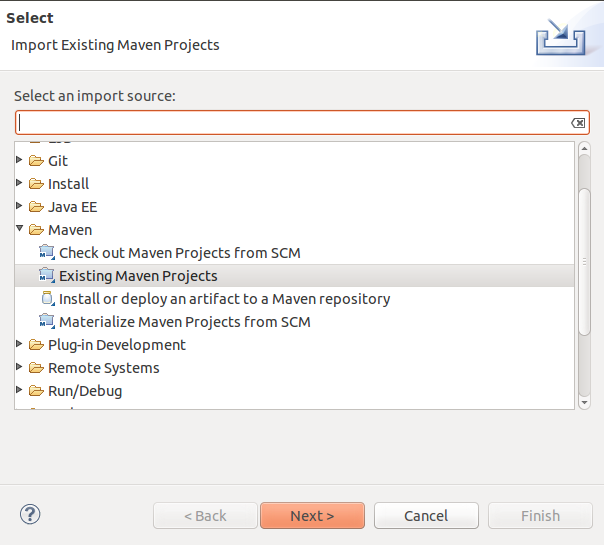
\includegraphics[width=0.6\textwidth]{./Figures/importdialog.png}
    \caption{Shown dialog after clicking on \textit{File > Import...} inside Eclipse.}
    \label{fig:importdialog}
  \end{center}
\end{figure}

Click on \textit{Existing Maven Projects} and \textit{Next}. Then \textit{Browse...} the folder where the project is stored. Finally, click \textit{Next} and \textit{Finish}. For running projects with Maven, you must right-click on the project, and then go to \textit{Run As > Maven clean}, as it is shown in Figure \ref{fig:RunAs}. In the console, you will see a ``BUILD SUCESS'', and then, repeat going to \textit{Run As > Maven install}. Now we are ready to import and run the client.

\begin{figure}
  \begin{center}
    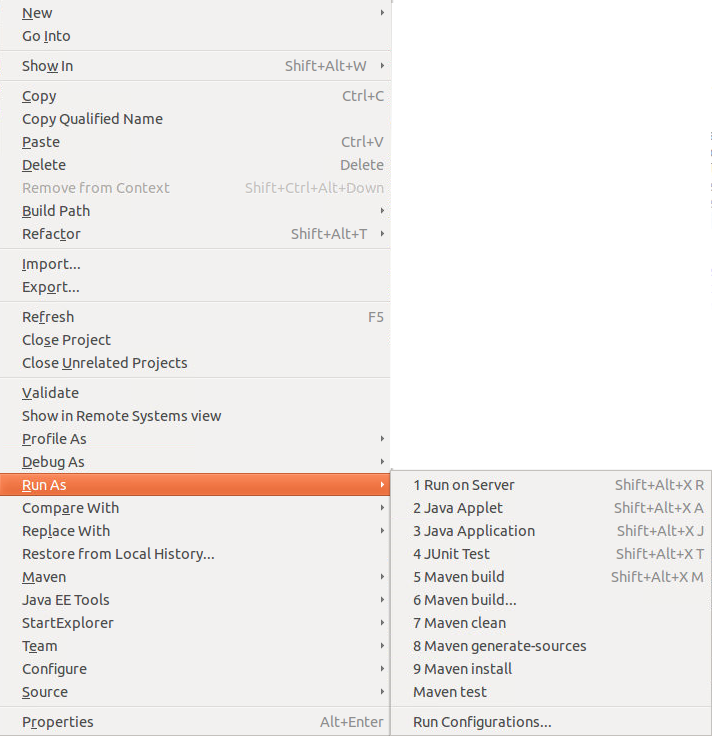
\includegraphics[width=0.65\textwidth]{./Figures/runAs.png}
    \caption{How to run a Maven project by making \textit{Run As > Maven clean}, and then \textit{Run As > Maven install}.}
    \label{fig:RunAs}
  \end{center}
\end{figure}

\section{Building Client application}
\label{sec:buildclient}



\chapter{Building MUSES Server}
\label{ch:server}

MUSES server has been developed using open source guidelines. It implements an Apache Tomcat server, and a MySQL database. This chapter describes all necessary steps to follow in order to build the server and run tests in it.

\section{Necessary tools and configuration}
\label{sec:serverpreliminaries}

First of all, and as MUSES server has been developed with Eclipse, these are the required tools to be able to finally build the server project. Therefore, the following are needed:

\begin{itemize}
  \item Eclipse, no specific version.
  \item Package \textit{Eclipse IDE for Java EE Developers}. To do this, there are two choices:
  \begin{enumerate}
    \item In Eclipse go to \textit{Help > Install New Software...}, and select the \textit{http://download.eclipse.org/releases/<youreclipsename>} in the \textit{Work with:} drop-down. Then look for \textit{Web, XML, Java EE and OSGi Enterprise Development} on the package list, and select it. Click \textit{Next} and \textit{Finish}, and restart Eclipse.
    \item The package is available at \url{https://eclipse.org/downloads/packages/eclipse-ide-java-ee-developers/lunasr2}, and the only thing to take into account is selecting the download according to your Eclipse version (name). On the website, simply select the correct one on ``Releases'', download it, and install it.
  \end{enumerate} 
  \item StartExplorer Eclipse plug-in. This plug-in is available at \url{http://basti1302.github.io/startexplorer/}, and you can just drag-and-drop the \textit{install} button on your Eclipse menu bar, or following the \textit{Help > Install New Software...} procedure.
\end{itemize}

Finally, as said in Section \ref{sec:musesgit}, \textit{MusesServer} files are located inside a repository of the MUSES organisation in GitHub (\url{https://github.com/MusesProject}). You can either download it as a ZIP file, or simply clone or fork the repository. For more information about Git, please refer to GitHub Help \cite{githelp:site}.

Before building the server project, MusesCommon project should be built. Please follow instructions of Section \ref{sec:common} before continue doing anything else.

\section{Bulding server project}
\label{sec:buildserver}

If Section \ref{sec:common} steps were successfully completed, we should have Maven correctly installed, and the MusesCommon project already builded. Now, the MusesServer project should be imported into the workspace in the same way, as a Maven project.

As the database is implemented on MySQL, we have to make sure that we have the \textit{mysql-connector-java} library properly installed. By right-clicking on the server project, at the end of the emerging window click on \textit{Properties}. The library should appear in the list which is in \textit{Java Build Path > Libraries tab}. If it does not appear, click \textit{Cancel} and in Eclipse, go to \textit{Window > Show view > Other...}. In the new window, inside the \textit{Java} folder, select \textit{Package Explorer} and then \textit{Ok}. A new tab will appear next to ``console'', ``error log'', ..., tabs. This tab shows the projects, like the \textit{Project Explorer} does. But in this view, we are able to use the \textit{StartExplorer} plug-in. By right-clicking in the MusesServer project, go to \textit{StartExplorer > Start Shell Here}, and a terminal will appear. If you cannot find this option, make sure that the \textit{StartExplorer} plug-in is installed (see Section \ref{sec:serverpreliminaries}). To obtain all the necessary configuration for managing MySQL databases and, in general, a Maven configuration for Eclipse, type into the terminal: \texttt{mvn eclipse:eclipse}. Wait for it to finish.

\subsection{Preparing the database}
\label{subsec:database}

The script for creating the MUSES server database is located at \texttt{MusesServer\\/db/startup\_db.sql}, and it should be loaded in the MySQL server at our machine. First, make sure you have MySQL server installed. If not, open a terminal and type \texttt{sudo apt-get install mysql-server-5.6}. During the installation, you will be asked to set a password for the root user. Few basic steps \cite{mysqlguide:site} should be followed to load the MUSES database:

\begin{description}
  \item[\texttt{root \#/etc/init.d/mysql start}] 
  \item[\texttt{user \$mysql -u root -h localhost -p}] and then enter the chosen password.
  \item[\texttt{SOURCE /home/yourusername/foldertoMusesServer/db/startup\_db.sql;}] which loads the database structure from the script.
  \item[\texttt{SOURCE /home/yourusername/foldertoMusesServer/db/startup\_db.sql;}] which populates the loaded database.
  \item[\texttt{SHOW DATABASES;}] should list the databases, and also MUSES database.
  \item[\texttt{USE muses;}]
  \item[\texttt{SHOW TABLES;}] should list the tables inside MUSES database.
  \item[\texttt{GRANT ALL ON muses.* TO 'muses'@'localhost';}] which gives permission to the MusesServer project to access the content in the MUSES database.
\end{description}

Finally, go to Eclipse again, right-click on the MusesServer project, and then go to \textit{Run As > Maven clean}, as it was shown in Figure \ref{fig:RunAs}. In the console, you will see a ``BUILD SUCESS'', and then, repeat going to \textit{Run As > Maven install}. Check that there were no errors, specially this type of error: \texttt{\textit{Error calling Driver\#connect}}, which means that the code cannot connect to the database. Now, you can implement functionalities and test them by doing \textit{Run As > Maven install} or \textit{Run As > Maven test}.

\chapter{Creating and integrating new sensors}
\label{ch:sensors}


\chapter{Installing MUSES}
\label{ch:installmuses}

\bibliographystyle{abbrv}
\bibliography{MUSESDevGuide}

\end{document}
